\documentclass[twoside,11pt]{article}
\usepackage{xr}
\usepackage[preprint]{jmlr2e}
\usepackage{times}
\usepackage{amsmath,mathtools,booktabs,microtype,enumitem}
\usepackage{lastpage}
\externaldocument[main-]{main}
\hypersetup{hidelinks,
pdftitle={Supplement: A Hierarchy of Risk Certificates for Forecasting Representations},
pdfauthor={Mohit Kumar and Somayeh Kargaran}}
\jmlrheading{}{2026}{1--\pageref{LastPage}}{}{}{}{Mohit Kumar and Somayeh Kargaran}
\ShortHeadings{Risk Certificates: Experimental Supplement}{Kumar and Kargaran}
\firstpageno{1}
\allowdisplaybreaks
\setlength{\emergencystretch}{1.5em}
\renewcommand{\thesection}{S\arabic{section}}
\renewcommand{\thetable}{S\arabic{table}}
\renewcommand{\thefigure}{S\arabic{figure}}
\renewcommand{\theequation}{S\arabic{equation}}

\begin{document}
\title{Supplement to A Hierarchy of Risk Certificates\\for Forecasting Representations}
\author{\name Mohit Kumar \email mohit.kumar@uni-rostock.de\\
\addr University of Rostock, Rostock, Germany\\
Software Competence Center Hagenberg, Hagenberg, Austria
\AND
\name Somayeh Kargaran \email somayeh.kargaran@scch.at\\
\addr Software Competence Center Hagenberg, Hagenberg, Austria}
\maketitle

\begin{abstract}
This supplement preserves the complete secondary experimental exposition and
the inherited local KAHM reconstruction equations accompanying the main
manuscript. It includes all finite-support lower-bound comparisons, the
explicit-feature decision control, full forecasting tables, preprocessing
comparisons, matched geometries and decoders, and speech-energy evidence.
Adverse and inconclusive outcomes are retained. All proofs of the main
paper's stated results remain in the main PDF. The repository supplies frozen
configurations, individual outcomes, exact source snapshots, and reproduction
commands for each separately defined study.
\end{abstract}

\paragraph{Reading conventions.}
Sections, tables, figures, and equations in this supplement have an S prefix.
References without that prefix refer to the main paper. Historical studies
retain their original designs and confidence allocations. Repeated fitting
on a previously examined natural-data cohort is descriptive; it does not
create an independent confirmation sample. The source-generation step only
expands the retained TeX inputs and resolves cross-document references.

% Generated by scripts/build_manuscript.py from sections/supplement_kahm_implementation.tex.
% Edit the source, then regenerate; all outcomes are retained.
\section{Local KAHM reconstruction implementation}
\label{supp:kahm-implementation}

This section records the inherited local reconstruction procedure used by the
forecasting implementation. It is supplied for reproducibility; the manuscript's
risk hierarchy requires the resulting fixed representation and metric, rather
than this particular reconstruction algorithm. The notation follows the main
paper: $z(x)\in\mathbb R^{d_x}$ is the training-preprocessed history, and
$\widehat z_{bcj}(x)$ is the reconstruction from local model $j$ in group $c$
of retained dictionary block $b$.

For one such local model, suppress the indices $(b,c,j)$ and write its
$N_{\rm loc}\geq2$ reference histories as
$z_1,\ldots,z_{N_{\rm loc}}\in\mathbb R^{d_x}$, with at least one direction of
nonzero empirical variance. The fitted linear encoding
$P\in\mathbb R^{r\times d_x}$ maps histories to
$r\geq1$ principal-component coordinates. The encoding retains only principal-component directions with positive empirical
variance. Let $\Sigma\in\mathbb R^{r\times r}$ be the resulting nonsingular
sample covariance of the encoded references. The Gaussian
kernel, its reference Gram matrix, and its query vector are
\begin{align*}
 k(\xi,\xi')&=\exp\!\left\{-\frac{(\xi-\xi')^\top\Sigma^{-1}
                                  (\xi-\xi')}{2r}\right\},\\
 K_{i\ell}&=k(Pz_i,Pz_\ell),\qquad
 k_x=(k(Pz_i,Pz(x)))_{i=1}^{N_{\rm loc}}.
\end{align*}
Here $\xi,\xi'\in\mathbb R^r$. For the local regularization parameter
$\eta>0$, kernel regression gives
$h(x)=(K+\eta I_{N_{\rm loc}})^{-1}k_x\in\mathbb R^{N_{\rm loc}}$.
Its coordinate $h_i$ uses regression targets equal to one at reference $i$
and zero at the other references. The reconstruction and its normalizer are
\begin{align*}
 s(x)&=\sum_{i=1}^{N_{\rm loc}}h_i(x),\qquad
 \widetilde s(x)=
 \begin{cases}s(x),&s(x)\ne0,\\1,&s(x)=0,\end{cases}\\
 \widehat z(x)&=\sum_{i=1}^{N_{\rm loc}}
                   \frac{h_i(x)}{\widetilde s(x)}z_i.
\end{align*}
The local regularization parameter also depends on the preprocessed values.
Collect the reference histories in the matrix
$Z=[z_1,\ldots,z_{N_{\rm loc}}]$ of size $d_x\times N_{\rm loc}$,
and let $v_z=\|Z\|_{\rm F}^2/(d_xN_{\rm loc})$. Starting at
$\eta_0=5v_z/2$, the implementation computes
\[
 B_k=(K+\eta_k I_{N_{\rm loc}})^{-1},\qquad
 \eta_{k+1}=2v_z+
       \frac{\|Z-ZKB_k\|_{\rm F}^2}{d_xN_{\rm loc}}.
\]
It stops when $|\eta_{k+1}-\eta_k|\leq10^{-3}$ or after 100 iterations,
and retains the last computed $B_k$; thus $\eta=\eta_k$ in the query map
above. Nonzero empirical variation implies $v_z>0$, so every inverse uses
positive regularization. This parameter is separate from the
forecast-decoder ridge parameter below.
When $s(x)\ne0$, the reconstruction coefficients sum to one and may be signed,
so $\widehat z(x)$ is an affine combination of reference histories. The
zero-sum convention defines the implementation at all queries but need not
preserve this affine-combination property.


The main paper defines the radial and angular folding score and the stable
normalized associations from these reconstructed histories. All local reference
sets, encodings, covariance matrices, and regularizers are fitted on development
data and frozen before calibration.

% Generated by scripts/build_manuscript.py from sections/witness_experiments.tex.
% Edit the source, then regenerate; all outcomes are retained.
\section{Lower-bound comparisons beyond two atoms}
\label{sec:witness-comparison}

The two-atom law in Proposition~\ref{main-prop:two-atom} has an exact population
witness. To distinguish a loose population bound from finite-sample uncertainty,
we evaluate eight finite-support distributions (Table~\ref{tab:witness-laws}).
They include deterministic and noisy targets, histories assigned identical
features despite different targets, rare conflicting targets, and a case in
which affine decoders are less expressive than general Lipschitz decoders.
For every method, $R^*$ is the minimum MSE over the same full scalar
$1$-Lipschitz class with outputs in $[-1,1]$. These explicit representations
isolate the behavior of the certificates;
they do not measure the forecasting accuracy of learned KAHM features.

\begin{table}[t]
\centering\footnotesize
\setlength{\tabcolsep}{3pt}
\begin{tabular}{llll}
\toprule
Law & Representation values $u_i$ & Targets $y_i$ & Stratum labels $c(u_i)$ \\
\midrule
Collapsed binary & $(0,0)$ & $(-1,1)$ & $(0,0)$ \\
Two atoms & $(-.6/\sqrt2,.6/\sqrt2)$ & $(-1,1)$ & $(0,0)$ \\
Three-point V & $(-1,0,1)$ & $(1,-1,1)$ & $(0,0,1)$ \\
Five-point zigzag & $(-1,-.5,0,.5,1)$ & $(-1,1,-1,1,-1)$ & $(0,0,1,1,1)$ \\
Partial collapse & $(-1,-1,0,0,1,1)$ & $(-1,.2,-.2,.2,-.2,1)$ & $(0,0,1,1,2,2)$ \\
Noisy affine & $(-1,-1,0,0,1,1)$ & $(-1,0,-.5,.5,0,1)$ & $(0,0,1,1,2,2)$ \\
Rare conflict & $(3,0,1)$ & $(0,-1,1)$ & $(0,1,1)$ \\
Affine mismatch & $(-1,0,1)$ & $(-.5,.5,-.5)$ & $(0,0,0)$ \\
\bottomrule
\end{tabular}
\caption{Prespecified joint supports for the lower-bound comparison. Entry $i$ gives one possible pair $(U,Y)=(u_i,y_i)$. Each row assigns equal probabilities to its entries, except rare conflict, whose probabilities are $(.9,.05,.05)$. Repeated representation values retain different possible targets. Stratum labels depend only on $U$ and are fixed before calibration. Every law uses $|u-u'|$, $\kappa=1$, and predictions in $[-1,1]$.}
\label{tab:witness-laws}
\end{table}


\paragraph{Protocol and comparators.}
The protocol was recorded before sampling. Each law uses 300 independent
calibration samples at each $n\in\{64,256,1024,4096\}$, totaling 9,600 trials.
The four primary methods share each sample and each receive a separate
one-sided failure probability $0.05$; no joint $95\%$ event across methods
is asserted. We compare the disjoint-pair empirical Bernstein (EB) bound in
Theorem~\ref{main-thm:episode-certificate}, the range-aware centered bound in
Appendix~\ref{main-app:centered-range-aware}, the dual-certified empirical risk
minimization (ERM) bound with Kullback--Leibler (KL) correction in
\eqref{main-eq:erm-kl-lower}, and the
stratified certificate in Theorem~\ref{main-thm:stratified-certificate}.
The primary stratified method estimates the stratum probabilities from the
calibration data. Both primary pairwise methods use the generic score range
$[0,2]$, obtained from a target diameter of two.
Prespecified secondary analyses tighten this range using the known support,
use known stratum masses, or replace the empirical-minimum correction by
Hoeffding's bound. The result archive includes every secondary analysis.

The empirical and population optimization programs use the full Lipschitz
class, with global extension from the finite support. Feasible primal and dual
values bracket each optimum; the largest empirical gap is
$4.01\times10^{-11}$. Analytic checks cover all eight population optima.
An unprojected affine optimum is never used as a Lipschitz lower bound: in the
mismatch law, the former is $2/9$ and the latter is zero.

\begin{table}[t]
\centering\small
\setlength{\tabcolsep}{3pt}
\begin{tabular}{lrrrrrrrr}
\toprule
& \multicolumn{4}{c}{Population quantities} & \multicolumn{4}{c}{Mean lower endpoint, $n=4096$} \\
\cmidrule(lr){2-5}\cmidrule(lr){6-9}
Law & $R^*$ & $W$ & $W_{\rm str}$ & $C$ & Pair & Centered & ERM & Strat. \\
\midrule
Collapsed binary & 1.0000 & 1.0000 & 1.0000 & 1.0000 & 0.9306 & 0.9149 & 0.9345 & 0.9237 \\
Two atoms & 0.3315 & 0.3315 & 0.3315 & 0.3315 & 0.3034 & 0.2807 & 0.2908 & 0.3001 \\
Three-point V & 0.2222 & 0.2222 & 0.1667 & 0.0160 & 0.1996 & 0.0000 & 0.1890 & 0.1355 \\
Five-point zigzag & 0.5400 & 0.3800 & 0.5250 & 0.0744 & 0.3408 & 0.0186 & 0.4891 & 0.4442 \\
Partial collapse & 0.2533 & 0.0867 & 0.2533 & 0.0000 & 0.0646 & 0.0000 & 0.2178 & 0.1772 \\
Noisy affine & 0.2500 & 0.0972 & 0.2500 & 0.0000 & 0.0777 & 0.0000 & 0.2145 & 0.1801 \\
Rare conflict & 0.0250 & 0.0025 & 0.0250 & 0.0000 & 0.0000 & 0.0000 & 0.0148 & 0.0059 \\
Affine mismatch & 0.0000 & 0.0000 & 0.0000 & 0.0000 & 0.0000 & 0.0000 & 0.0000 & 0.0000 \\
\bottomrule
\end{tabular}
\caption{Finite-support comparison on the same full scalar Lipschitz class. $R^*$ is the minimum MSE, $W$ the unconditional pair witness, $W_{\rm str}$ the prespecified stratified witness, and $C$ the centered population bound. The last four columns average 300 independent calibration samples. Each method separately has nominal one-sided confidence $95\%$; no joint confidence across columns is asserted. Empirical risk minimization (ERM) uses a dual-certified empirical minimum and bounded-loss Kullback--Leibler (KL) inversion. Primary stratification estimates the stratum masses. All quantities are in MSE units.}
\label{tab:witness-comparison}
\end{table}


\paragraph{Population slack and finite-sample cost.}
Table~\ref{tab:witness-comparison} reports population quantities separately
from mean calibrated endpoints. On partial collapse, stratification raises
the population witness from $0.0867$ to the exact minimum $0.2533$.
At $n=4096$, its mean endpoint is $0.1772$, compared with $0.0646$ for
unconditional pairing and $0.2178$ for empirical minimization. Stratification
also improves the five-point and noisy-affine witnesses. It worsens the
three-point witness, from $0.2222$ to $0.1667$, demonstrating that a fixed
partition need not help.

Empirical minimization gives the largest mean endpoint on most richer laws;
the pair bound is larger on the partially separated two-atom and three-point
laws at $n=4096$. Accounting for a known representation range substantially
improves centered calibration when the representation is constant.
The two-atom comparison in Section~\ref{sec:experiments}
quantifies how treating a known zero variance as unknown can weaken a centered
endpoint. Consequently, the relative performance of pairwise and centered
certificates depends on the estimator and the structural information supplied
to it.

\begin{figure}[p]
\centering
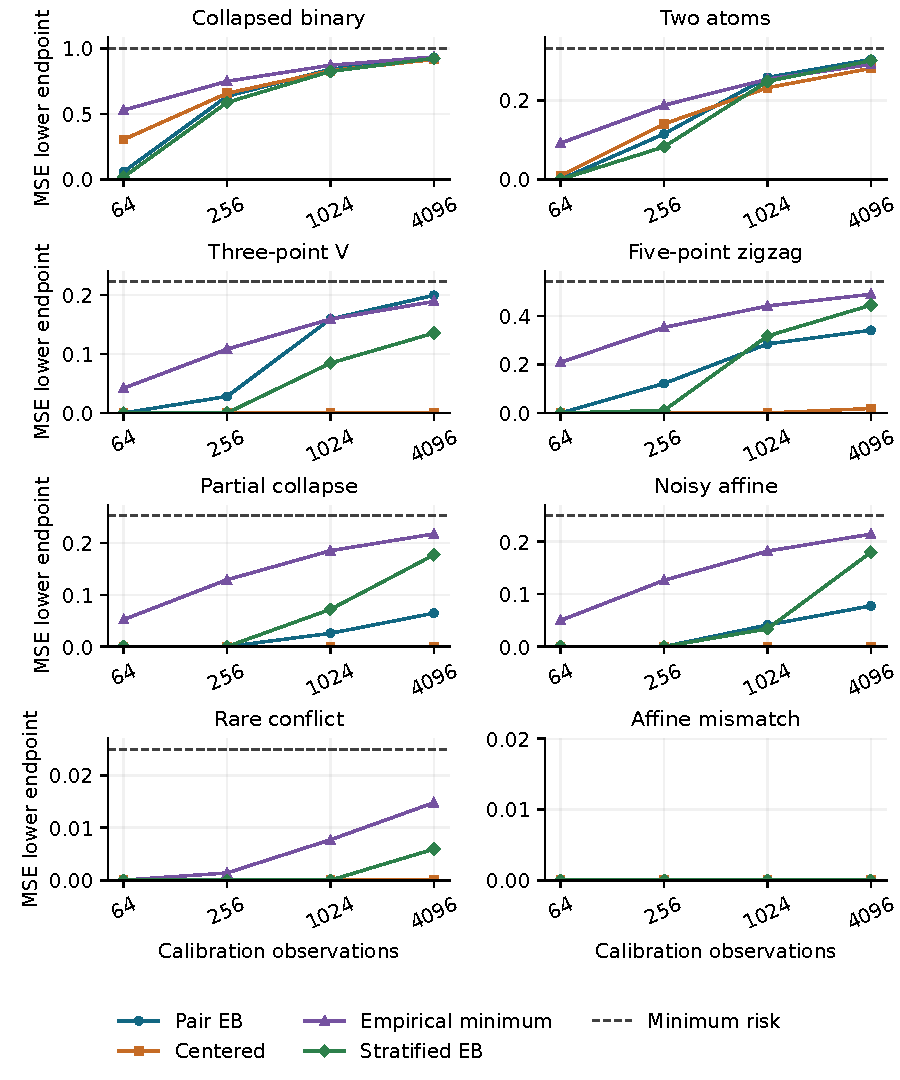
\includegraphics[width=\linewidth]{figures/witness_sample_size.pdf}
\caption{Mean lower endpoints over all 300 repetitions at each calibration
size for every prespecified law. Dashed lines show minimum population MSE.
Each method has its own $95\%$ one-sided confidence statement. The result
archive provides endpoint quantiles, Monte Carlo confidence
intervals, secondary methods, and all individual trials.}
\label{fig:witness-sample-size}
\end{figure}

\paragraph{Positive tolerances, coverage, and computation.}
The fixed RMSE tolerances are $0.10$, $0.25$, and $0.50$ for every law.
On partial collapse at $n=4096$, unconditional pairing excludes tolerance
$0.25$ in 211 of 300 trials; empirical minimization and primary stratification
both exclude it in all 300. Rare conflicts remain difficult: their exact
risk is $0.025$, but unconditional pairing and primary stratification never
exclude tolerance $0.10$ at this sample size. Empirical minimization excludes
it in all 300 trials. Tightening the stratified score range using the known
support raises its exclusion count to 284; additionally supplying known masses
raises it to 300. The gain therefore depends on both pairing and available
information.

All four primary methods have zero observed coverage violations across the
prespecified grid. This simulation does not prove coverage; each law--size
cell has only 300 repetitions, and the result archive gives binomial Monte
Carlo confidence intervals. At $n=4096$, medians across the eight
law-wise median computation times are $31.3$, $34.7$, $265.4$, and $165.0$
$\mu$s for pair EB, centered, empirical minimum, and stratified EB,
respectively. These single-machine measurements use a precomputed finite-support
pair-score table and include sample statistics, confidence corrections, and
ERM optimization after representation lookup. They exclude feature learning
and do not establish a computational advantage on large continuous supports.
The frozen protocol, sufficient statistics, dual certificates, and complete
analysis are in \path{results/witness_comparison}.

% Generated by scripts/build_manuscript.py from sections/archive/decision_value_detailed.tex.
% Edit the source, then regenerate; all outcomes are retained.
\section{Decisions at a positive error tolerance}
\label{sec:decision-value}

\paragraph{Decisions in the KAHM forecasting studies.}
The main synthetic, oscillator, and coefficient-budget studies contain 62
fitting runs (Sections~\ref{sec:experiments}--\ref{sec:budget-sensitivity}).
We distinguish exclusion of a candidate's decoder class from the behavior
of a model selected by validation. Among the 800 main-study candidates, the all-horizon decisions at
RMSE tolerance $0.35$ are 301 accepted, 24 excluded, and 475 unresolved;
the corresponding oscillator counts are 55, 30, and 155 among 240 candidates.
Nevertheless, all 186 horizon-specific lower endpoints of the 62 models
selected by validation across the complete candidate family are zero.
Restricting validation selection to retained KAHM gives 184 zero endpoints
out of 186. These descriptive counts motivate a separate test of whether
lower certificates can resolve a decision that upper calibration leaves open.

\paragraph{A controlled forecasting mechanism.}
The protocol is specified before calibration observations are generated.
Each independent episode supplies one history $X=(Z,S)$ and one scalar future
$Y$. The indicator $S$ equals one with probability $0.2$ and zero otherwise,
and $Z,R,N$ are mutually independent random signs, each taking $-1$ and $1$
with equal probability, independently of $S$. We consider two regimes, called
repairable and irreducible because the final
representation can remove the signal uncertainty only in the first:
\[
  Y=0.8SZ+0.1N \quad\text{(repairable)},\qquad
  Y=0.8SR+0.1N \quad\text{(irreducible)}.
\]
The three entries of $(Z,S,Y)$ occur in temporal order, and the forecast is
made after observing $Z$ and $S$, before observing $Y$. The target range is
$[-0.9,0.9]$. We append the simplex
blocks
\[
 (1),\qquad (1-S,S),\qquad
 \bigl((1+SZ)/2,(1-SZ)/2\bigr)
\]
under the common coefficient budget $\kappa=2$. The first block has one
coordinate; the first two have three coordinates in
total; and all three have five. These coordinate counts define the costs
$1,3,5$ of the three representation classes. These explicit representations
test the general theorem; they are not fitted KAHM dictionaries.

At costs $1$, $3$, and $5$, the exact minimum MSEs in the repairable regime
are $0.138$, $0.138$, and $0.01$. They all equal $0.138$ in the irreducible
regime. In the former, the last
block represents the conditional mean $0.8SZ$ with coefficients
$(0.8,-0.8)$, whose norm is below $2$. In the latter, the unobserved sign $R$
leaves the conditional mean zero even with the complete history. The prescribed
RMSE tolerance $0.30$ therefore requires the last prefix in one regime and
is unattainable in the other. For the cost-$3$ prefix, the unconditional
population witness is only $0.0324$, whereas pairing conditionally on $S$
gives $0.138$. This isolates a population limitation of unconditional pairing,
in addition to finite-sample uncertainty.

\paragraph{Calibration and comparisons.}
Each of 100 independent repetitions per regime uses 2,048 training episodes,
1,024 validation episodes, and nested calibration samples of
$256,1024,4096,16384,65536$ episodes. All three decoders are fitted with zero
ridge penalty and frozen before calibration. The RMSE tolerance $0.30$
corresponds to an MSE threshold of $0.09$. We compare validation-only
acceptance at this threshold, calibrated upper-bound acceptance, and two
extensions of the latter rule using either unconditional or stratified
lower certificates.
Validation-only acceptance is a descriptive reference rule without a population
confidence guarantee. The two predefined partitions use the history labels
$S$ and $(S,Z)$; neither
partition uses the future target. For the latter method, we estimate
stratum masses and take the maximum of the two separately budgeted endpoints
from Theorem~\ref{main-thm:stratified-certificate}. One failure budget $0.05$ per
regime and repetition covers all prefixes and all five sample sizes:
$0.02$ for upper bounds, $0.01$ for unconditional lower bounds, and $0.02$
for both stratified families. Calibration uses one forecast per independent
episode; it does not treat dependent windows as independent observations.

\begin{table}[t]
\centering
\small
\begin{tabular}{rccccc}
\toprule
 & \multicolumn{3}{c}{Repairable regime} & \multicolumn{2}{c}{Irreducible regime} \\
\cmidrule(lr){2-4}\cmidrule(lr){5-6}
$n$ & Upper & \multicolumn{2}{c}{Minimum cost $5$} & \multicolumn{2}{c}{All classes excluded} \\
 & acceptance & Unconditional & Stratified & Unconditional & Stratified \\
\midrule
256 & 0 & 0 & 0 & 0 & 0 \\
1,024 & 100 & 0 & 0 & 0 & 0 \\
4,096 & 100 & 0 & 0 & 0 & 0 \\
16,384 & 100 & 0 & 100 & 0 & 1 \\
65,536 & 100 & 0 & 100 & 0 & 100 \\
\bottomrule
\end{tabular}
\caption{Decision counts out of 100 independent repetitions in each constructed regime, at the prespecified RMSE tolerance $0.30$. Upper acceptance certifies a fitted predictor; equality of the cost endpoints certifies the least feasible cost among the three predefined classes. The unconditional and stratified methods share the same upper endpoint and fitted model. Every irreducible-regime upper decision is unresolved. One failure budget $0.05$ covers all five calibration sizes and all reported endpoints within each regime and repetition.}
\label{tab:decision-outcomes}
\end{table}


\paragraph{Decision value and sample requirements.}
Validation accepts the repaired cost-$5$ model in all 100 repetitions, and
upper calibration does so from $n=1024$ onward. Stratified lower certificates
exclude both cheaper classes in all repetitions at $n=16384$ and $65536$,
so the cost interval in Corollary~\ref{main-cor:cost-optimality} reduces to
$[5,5]$. Unconditional lower calibration never closes this interval at the
prescribed sample sizes. Both procedures select the same accepted predictor;
the additional conclusion is that no cheaper prescribed class can meet the
tolerance, independently of its decoder optimization.

The irreducible control produces no upper acceptance. Stratified lower
calibration excludes all three classes in 1 of 100 repetitions at $n=16384$
and all 100 at $n=65536$; unconditional lower calibration never excludes all
three. Small samples reveal the cost of stratification: at $n=4096$,
unconditional pairing excludes the constant class in every repetition of
both regimes, while the stratified method excludes no class. All 600 fits
converged, and the exact population risks satisfy every reported simultaneous
interval event in all 200 regime--repetition instances. The experiment
demonstrates a class-level decision under a controlled mechanism, with
substantial sample requirements; it does not establish its frequency in
natural forecasting tasks.

\begin{figure}[t]
\centering
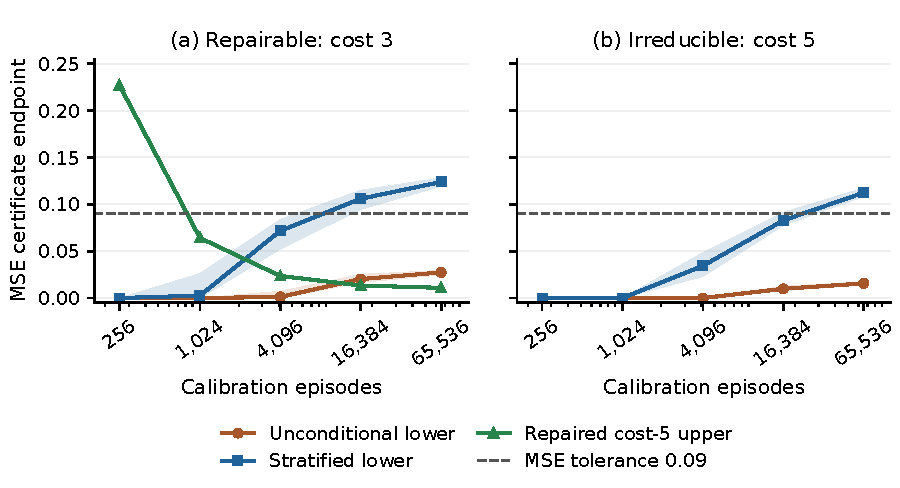
\includegraphics[width=\linewidth]{figures/decision_endpoints.pdf}
\caption{Calibration-size dependence in the constructed decision experiment.
Lines show medians and shaded bands the full range across 100 independent
repetitions; the bands describe repetition variability. Panel (a) compares
lower endpoints for the inadequate cost-$3$ class with the upper endpoint
for the repaired cost-$5$ predictor. Panel (b) shows lower endpoints for the
most detailed class in the irreducible regime. The dashed line is the fixed
MSE tolerance $0.09$.}
\label{fig:decision-endpoints}
\end{figure}

% Generated by scripts/build_manuscript.py from sections/experiments.tex.
% Edit the source, then regenerate; all outcomes are retained.
\section{KAHM forecasting on bounded synthetic systems}
\label{sec:experiments}

The preceding studies test the general risk certificates. This section applies
the KAHM learner to four bounded forecasting systems. The comparison includes
all prescribed configurations. Empirical test error describes performance on
a held-out sample; a certified risk endpoint bounds the corresponding
population expectation under the stated sampling assumptions.

\subsection{Protocol and predictive accuracy}

Four generators produce independent length-72 episodes: a noisy harmonic
oscillator, a quasiperiodic signal, nonlinear autoregression with bounded
innovations, and a logistic map with an episode-specific parameter. Their
observations lie in $[-1,1]$ by construction
(Appendix~\ref{app:protocols}). Each of five fitting repetitions uses 128
training, 512 validation, 4096 calibration, and 2048 test episodes. Histories
have lengths $m\in\{4,12\}$, horizons are $\{1,4,12\}$, and the 13 common
zero-based origins are $11,15,\ldots,59$. Within-episode windows may be
dependent. Geometry is relearned in each repetition, with budget $\kappa=4$,
ridge coefficient $10^{-4}$, affinity exponent $16$, and prefix dimensions
$2,6,14,30$. Geometry fitting uses at most 1600 histories and 24 local points.

Each repetition freezes 40 candidates: retained KAHM, RBF, and affine-hull
features; hard KAHM assignments; ordinary Frobenius-budget and exact-duplicate
ablations; ridge autoregression (AR); quadratic regression; KAHM and polynomial
feature rollouts; persistence; and a constant model. One candidate per family
is selected by validation MSE across horizons. These specified configurations
assess the procedure, rather than the best possible tuning of each family.

The failure budget $0.05$ per repetition allocates $0.04$ across
$2\times40\times3$ one-sided risk bounds and $0.01$ across 18 adjacent-prefix
improvement comparisons. Upper bounds use 4096 episode losses; lower bounds
use 2048 disjoint episode pairs. The 13 origins do not increase these independent
sample sizes. The joint event is per complete repetition, not across all runs.

\begin{table}[t]
\centering\small
\setlength{\tabcolsep}{3pt}
\begin{tabular}{lrrrrrrrr}
\toprule
& \multicolumn{2}{c}{Harmonic} & \multicolumn{2}{c}{Quasiperiodic} & \multicolumn{2}{c}{Nonlinear AR} & \multicolumn{2}{c}{Logistic}\\
Method & $h=1$ & $h=12$ & $h=1$ & $h=12$ & $h=1$ & $h=12$ & $h=1$ & $h=12$\\
\midrule
KAHM blocks & \shortstack[r]{0.070\\(0.001)} & \shortstack[r]{0.346\\(0.006)} & \shortstack[r]{0.078\\(0.003)} & \shortstack[r]{0.284\\(0.004)} & \shortstack[r]{0.054\\(0.001)} & \shortstack[r]{0.074\\(0.001)} & \shortstack[r]{0.176\\(0.018)} & \shortstack[r]{0.511\\(0.001)}\\[2pt]
RBF blocks & \shortstack[r]{0.068\\(0.001)} & \shortstack[r]{0.351\\(0.003)} & \shortstack[r]{0.068\\(0.005)} & \shortstack[r]{0.287\\(0.004)} & \shortstack[r]{0.057\\(0.001)} & \shortstack[r]{0.074\\(0.001)} & \shortstack[r]{0.172\\(0.012)} & \shortstack[r]{0.512\\(0.001)}\\[2pt]
Affine-hull blocks & \shortstack[r]{0.072\\(0.003)} & \shortstack[r]{0.357\\(0.004)} & \shortstack[r]{0.110\\(0.007)} & \shortstack[r]{0.275\\(0.006)} & \shortstack[r]{0.059\\(0.003)} & \shortstack[r]{0.074\\(0.001)} & \shortstack[r]{0.156\\(0.014)} & \shortstack[r]{0.509\\(0.001)}\\[2pt]
Hard KAHM states & \shortstack[r]{0.097\\(0.003)} & \shortstack[r]{0.358\\(0.003)} & \shortstack[r]{0.127\\(0.002)} & \shortstack[r]{0.300\\(0.006)} & \shortstack[r]{0.062\\(0.001)} & \shortstack[r]{0.074\\(0.001)} & \shortstack[r]{0.235\\(0.005)} & \shortstack[r]{0.512\\(0.001)}\\[2pt]
Ridge AR & \shortstack[r]{0.038\\(0.000)} & \shortstack[r]{0.281\\(0.004)} & \shortstack[r]{0.033\\(0.000)} & \shortstack[r]{0.259\\(0.002)} & \shortstack[r]{0.047\\(0.000)} & \shortstack[r]{0.080\\(0.001)} & \shortstack[r]{0.409\\(0.002)} & \shortstack[r]{0.507\\(0.002)}\\[2pt]
Quadratic regression & \shortstack[r]{0.031\\(0.000)} & \shortstack[r]{0.243\\(0.003)} & \shortstack[r]{0.030\\(0.000)} & \shortstack[r]{0.246\\(0.002)} & \shortstack[r]{0.047\\(0.000)} & \shortstack[r]{0.081\\(0.001)} & \shortstack[r]{0.010\\(0.000)} & \shortstack[r]{0.508\\(0.003)}\\[2pt]
KAHM rollout & \shortstack[r]{0.070\\(0.002)} & \shortstack[r]{0.358\\(0.004)} & \shortstack[r]{0.079\\(0.004)} & \shortstack[r]{0.319\\(0.011)} & \shortstack[r]{0.055\\(0.001)} & \shortstack[r]{0.074\\(0.001)} & \shortstack[r]{0.174\\(0.018)} & \shortstack[r]{0.524\\(0.004)}\\[2pt]
Polynomial rollout & \shortstack[r]{0.030\\(0.000)} & \shortstack[r]{0.297\\(0.010)} & \shortstack[r]{0.030\\(0.000)} & \shortstack[r]{0.288\\(0.004)} & \shortstack[r]{0.047\\(0.000)} & \shortstack[r]{0.084\\(0.003)} & \shortstack[r]{0.010\\(0.000)} & \shortstack[r]{0.502\\(0.004)}\\[2pt]
Persistence & \shortstack[r]{0.125\\(0.000)} & \shortstack[r]{1.085\\(0.004)} & \shortstack[r]{0.084\\(0.000)} & \shortstack[r]{0.743\\(0.004)} & \shortstack[r]{0.055\\(0.000)} & \shortstack[r]{0.103\\(0.001)} & \shortstack[r]{0.931\\(0.006)} & \shortstack[r]{0.661\\(0.006)}\\[2pt]
\bottomrule
\end{tabular}
\caption{Independent-test RMSE: mean over five complete fitting repetitions, with sample standard deviation below in parentheses. One candidate per family is selected by validation MSE across all three horizons before calibration or test scoring. The archive includes $h=4$, all candidates, and every confidence endpoint. Fitting variation differs from uncertainty conditional on a fitted model; these test errors are descriptive estimates.}
\label{tab:forecast}
\end{table}


Table~\ref{tab:forecast} includes variation across the five fits. KAHM improves
substantially over long-horizon persistence on the periodic generators, but
quadratic and autoregressive models are stronger there. On nonlinear AR,
KAHM horizon-12 RMSE is $0.0743$, compared with $0.0802$ for ridge AR and
$0.0813$ for quadratic regression; the latter families are better at horizon
one. Direct KAHM fitting improves on feature rollout at horizon 12 on the two
periodic generators. The independently initialized oscillators in Section~\ref{sec:oscillators}
show that direct fitting does not always outperform feature rollout.

\subsection{Acceptance, exclusion, and fitted refinement}

\begin{table}[t]
\centering\small
\begin{tabular}{lcccccc}
\toprule
& \multicolumn{3}{c}{KAHM retained family} & \multicolumn{3}{c}{All candidates}\\
System & $\epsilon=.20$ & $.35$ & $.50$ & $\epsilon=.20$ & $.35$ & $.50$\\
\midrule
Harmonic & 0/5 (--) & 0/5 (--) & 5/5 (6) & 0/5 (--) & 5/5 (12) & 5/5 (4)\\
Quasiperiodic & 0/5 (--) & 5/5 (14) & 5/5 (2) & 0/5 (--) & 5/5 (4) & 5/5 (1)\\
Nonlinear AR & 5/5 (2) & 5/5 (2) & 5/5 (2) & 5/5 (2) & 5/5 (2) & 5/5 (2)\\
Logistic & 0/5 (--) & 0/5 (--) & 0/5 (--) & 0/5 (--) & 0/5 (--) & 0/5 (--)\\
\bottomrule
\end{tabular}
\caption{Runs certifying the same RMSE tolerance at all horizons $1,4,12$. Parentheses give median retained feature dimension among successful least-dimension selections; `--' means no model passed. Cost is a representation-size proxy, not measured runtime. Each run has a joint 95\% event covering its complete frozen family and improvement comparisons.}
\label{tab:selection}
\end{table}


The retained KAHM family certifies the all-horizon RMSE requirement $0.20$
for every nonlinear-AR repetition, $0.35$ for every quasiperiodic repetition,
and $0.50$ for every harmonic repetition. Allowing all families also certifies
$0.35$ on harmonic data. No candidate certifies $0.50$ on the logistic task;
this is unresolved, not evidence that all true risks exceed the threshold.
Even the selected harmonic quadratic model's mean one-step test RMSE $0.0311$
corresponds to a mean upper endpoint $0.1497$, illustrating the precision cost.

Of 480 retained-KAHM candidate--horizon statements, 119 have positive lower
endpoints. Only two exclude RMSE $0.35$, and none excludes $0.50$; positive
endpoints alone are not enough for a useful positive-tolerance decision.
Section~\ref{sec:decision-value} compares the acceptance, exclusion, and
unresolved decisions across the forecasting studies.
Paired comparisons certify 72 of 360 adjacent-prefix improvements. Nonlinear
AR has no certified adjacent-prefix gain despite meeting useful tolerances.
The complete refinement curves and system-specific counts are retained in
the repository; nesting a class does not guarantee improvement of each fit.

Exact duplication is already covered analytically by
Theorem~\ref{main-thm:replication-invariance}. Zero-ridge numerical checks reproduce
matching minimum training risks within their solver gaps. The main duplicate
candidate uses zero ridge, whereas primary models use $10^{-4}$; their fitted
errors are therefore not evidence for ridge-estimator invariance.
All 800 main-study candidates completed; the constrained block fits have
recorded first-order optimality gaps below $10^{-7}$. These numerical
optimization guarantees are separate from the risk guarantees, which require
the sampling assumptions in Section~\ref{main-sec:theory}. Appendix~\ref{app:protocols}
describes reproduction of the fitted models and confidence endpoints.

\paragraph{Calibration on a two-atom distribution.}
A separate benchmark contains 28,800 trials with analytically known class
and fitted risks (Appendix~\ref{main-app:known-risk}). One pairwise lower endpoint
exceeds its true risk; no centered lower or fitted upper endpoint does.
The centered estimator in this benchmark estimates representation variance
even when that variance is known to be zero. At full collapse and $n=4096$,
its mean lower endpoint is $0.5327$. Substituting the known zero variance while
keeping the same target correction gives a lower bound of approximately
$0.9031$ on the expected endpoint; the pairwise method has mean endpoint $0.9177$. Thus part of the
observed difference is caused by unused structural information. The
$n^{-1/4}$ correction of this centered estimator is not a limitation of all
centered methods. Section~\ref{sec:witness-comparison} compares a method based
on direct standard-deviation concentration and a certified empirical minimum.

% Generated by scripts/build_manuscript.py from sections/oscillators.tex.
% Edit the source, then regenerate; all outcomes are retained.
\subsection{Independently initialized Van der Pol and Duffing episodes}
\label{sec:oscillators}

We apply the frozen 40-candidate procedure to independently initialized
Van der Pol and forced Duffing episodes, connecting the experiment to
\citet{kumar2026limits}. Each system has three new complete fits with the
sample sizes and confidence allocation of Section~\ref{sec:experiments}.
The bounded position sensor, dynamics, and numerical checks are specified in
Appendix~\ref{app:oscillator-protocol}. Horizons $1,4,12$ correspond to
$0.1,0.4,1.2$ time units. Certificates concern sensor-output error under the
independent-episode numerical law; they require neither stationarity nor
independent within-episode windows and do not certify physical-state error.

\begin{table}[t]
\centering\small
\setlength{\tabcolsep}{3pt}
% Generated by experiments/run_oscillators.py; no manually entered results.
\begin{tabular}{llrrrr}
\toprule
System & Family & $h=1$ & $h=4$ & $h=12$ & $\overline{\sqrt{U_{12}}}$ \\
\midrule
Van der Pol & KAHM blocks & $0.099\pm0.001$ & $0.139\pm0.005$ & $0.381\pm0.023$ & 0.409 \\
Van der Pol & RBF blocks & $0.106\pm0.005$ & $0.152\pm0.011$ & $0.383\pm0.010$ & 0.412 \\
Van der Pol & Affine blocks & $0.137\pm0.003$ & $0.192\pm0.006$ & $0.299\pm0.009$ & 0.333 \\
Van der Pol & Ridge AR & $0.038\pm0.000$ & $0.150\pm0.001$ & $0.353\pm0.001$ & 0.383 \\
Van der Pol & Quadratic direct & $0.032\pm0.000$ & $0.138\pm0.001$ & $0.342\pm0.001$ & 0.374 \\
Van der Pol & KAHM rollout & $0.034\pm0.012$ & $0.064\pm0.030$ & $0.341\pm0.033$ & 0.374 \\
Van der Pol & Quadratic rollout & $0.029\pm0.000$ & $0.127\pm0.002$ & $0.399\pm0.006$ & 0.427 \\
Van der Pol & Persistence & $0.089\pm0.000$ & $0.339\pm0.000$ & $0.868\pm0.001$ & 0.885 \\
Duffing & KAHM blocks & $0.080\pm0.002$ & $0.120\pm0.004$ & $0.250\pm0.010$ & 0.300 \\
Duffing & RBF blocks & $0.061\pm0.001$ & $0.098\pm0.003$ & $0.229\pm0.007$ & 0.281 \\
Duffing & Affine blocks & $0.064\pm0.004$ & $0.097\pm0.003$ & $0.223\pm0.005$ & 0.274 \\
Duffing & Ridge AR & $0.019\pm0.000$ & $0.041\pm0.000$ & $0.151\pm0.001$ & 0.214 \\
Duffing & Quadratic direct & $0.017\pm0.000$ & $0.035\pm0.000$ & $0.137\pm0.001$ & 0.203 \\
Duffing & KAHM rollout & $0.081\pm0.001$ & $0.126\pm0.004$ & $0.269\pm0.014$ & 0.315 \\
Duffing & Quadratic rollout & $0.017\pm0.000$ & $0.035\pm0.000$ & $0.140\pm0.002$ & 0.206 \\
Duffing & Persistence & $0.033\pm0.001$ & $0.114\pm0.002$ & $0.318\pm0.005$ & 0.363 \\
\bottomrule
\end{tabular}

\caption{Independent-test sensor RMSE, mean $\pm$ sample standard deviation
over three complete fits, with validation selection within each family.
The last column averages the selected models' individual horizon-12
upper-RMSE endpoints; this descriptive average gives no ensemble guarantee.
All 40 candidates per repetition are archived.}
\label{tab:oscillators}
\end{table}

Retained KAHM improves horizon-12 RMSE over persistence on Van der Pol
($0.3814$ versus $0.8677$) and Duffing ($0.2499$ versus $0.3185$), but other
models perform better: affine-hull blocks achieve $0.2990$ on Van der Pol,
and quadratic regression achieves $0.1369$ on Duffing
(Table~\ref{tab:oscillators}). Iterated KAHM achieves $0.3408$ on Van der Pol
and $0.2686$ on Duffing, so direct fitting outperforms iteration only on the
latter system.

Retained KAHM certifies all-horizon RMSE $0.35$ in all three Duffing fits
and $0.50$, but not $0.35$, in all three Van der Pol fits. Allowing all
comparison families certifies $0.35$ in every fit of both systems; none
certifies $0.20$. Adjacent KAHM refinements have positive certified improvement
in 43 of 54 Van der Pol comparisons and 10 of 54 Duffing comparisons.

% Generated by scripts/build_manuscript.py from sections/sensitivity.tex.
% Edit the source, then regenerate; all outcomes are retained.
\subsection{Sensitivity to the coefficient budget}
\label{sec:budget-sensitivity}

The budget $\kappa$ defines a feature-dependent class; equal numerical budgets
do not imply equal capacity across representations. To assess sensitivity to
this choice, a separate experiment uses fresh development, calibration, and
test streams with seeds 2701--2703, $m=12$, and $\kappa\in\{1,4,16\}$ on all
four main systems. Other settings match Section~\ref{sec:experiments}. The
design comprises 36 runs and 756 fitted models, with 21 candidates per
budget and system--seed combination. Budgets share streams and geometry
within each system--seed repetition. Validation selects a KAHM prefix
separately at each budget. Allocating $0.05/3$ to each budget's risk and
refinement bounds gives joint confidence at least $0.95$ across budgets
within a repetition, without a joint claim across all twelve repetitions.

\begin{table}[t]
  \centering
  \small
  \setlength{\tabcolsep}{4pt}
  % Automatically generated by experiments/run_sensitivity.py.
\begin{tabular}{llrrrrr}
\toprule
System & $\kappa$ & Features & $h=1$ & $h=4$ & $h=12$ & Passes \\
\midrule
Harmonic & 1 & 16.7 & 0.3737 & 0.4102 & 0.4696 & 0/3 \\
Harmonic & 4 & 30.0 & 0.1414 & 0.2313 & 0.3900 & 0/3 \\
Harmonic & 16 & 30.0 & 0.1392 & 0.2292 & 0.3875 & 0/3 \\
\addlinespace[2pt]
Quasiperiodic & 1 & 24.7 & 0.2510 & 0.2905 & 0.3336 & 0/3 \\
Quasiperiodic & 4 & 30.0 & 0.1294 & 0.2050 & 0.2927 & 3/3 \\
Quasiperiodic & 16 & 30.0 & 0.1294 & 0.2050 & 0.2927 & 3/3 \\
\addlinespace[2pt]
Nonlinear AR & 1 & 7.3 & 0.1059 & 0.1056 & 0.1068 & 3/3 \\
Nonlinear AR & 4 & 30.0 & 0.0670 & 0.0730 & 0.0746 & 3/3 \\
Nonlinear AR & 16 & 30.0 & 0.0670 & 0.0730 & 0.0746 & 3/3 \\
\addlinespace[2pt]
Logistic & 1 & 30.0 & 0.4713 & 0.5003 & 0.5052 & 0/3 \\
Logistic & 4 & 30.0 & 0.4384 & 0.4967 & 0.5044 & 0/3 \\
Logistic & 16 & 30.0 & 0.4384 & 0.4968 & 0.5044 & 0/3 \\
\bottomrule
\end{tabular}

  \caption{Budget sensitivity: mean test RMSE and feature count over three
  new fitting seeds. ``Passes'' counts validation-selected KAHM models
  certified at tolerance $0.35$ simultaneously for $h=1,4,12$. The confidence
  allocation covers all three budgets within each system--seed repetition.}
  \label{tab:budget}
\end{table}

Increasing $\kappa$ from 1 to 4 reduces one-step KAHM RMSE from $0.3737$ to
$0.1414$ on the harmonic system and from $0.1059$ to $0.0670$ on nonlinear
autoregression; quasiperiodic $0.35$ certification increases from zero to three
passes. Increasing it from 4 to 16 gives little further improvement:
harmonic horizon-12 RMSE changes from $0.3900$ to $0.3875$, with no $0.35$
pass; quasiperiodic and nonlinear-AR errors are unchanged at displayed
precision, and logistic horizon-12 RMSE remains about $0.5044$, without a pass.
This does not establish impossibility at larger budgets or richer geometries.

At $\kappa=16$, harmonic AR and quadratic baselines achieve horizon-12 RMSEs
$0.2377$ and $0.2375$ and certify $0.35$ in all three fits. On nonlinear
autoregression at $\kappa=4$, KAHM has lower horizon-12 RMSE ($0.0746$ versus
$0.0800$ and $0.0809$) but higher one-step error. Every constrained fit has
a first-order optimality gap below $10^{-7}$.

% Generated by scripts/build_manuscript.py from sections/real_data.tex.
% Edit the source, then regenerate; all outcomes are retained.
\subsection{Writer-disjoint forecasting of original pen trajectories}
\label{sec:pendigits}

We use the original, unnormalized PenDigits trajectories
\citep{alpaydin1996pendigits}; the archive's spatially resampled table uses
whole-character preprocessing unsuitable for causal forecasting. The known
coordinate range $[0,500]^2$ permits transforming each coordinate $z$ to
$z/250-1$ and clipping predictions to $[-1,1]$, without stroke-specific normalization.
Acquisition and development details are in Appendix~\ref{app:pendigits-protocol}.

Writer identifiers are inferred from the second integer in each UNIPEN
\texttt{COMMENT} field: their ranges and record counts agree with the
documented 30 development and 14 test writers, but the field semantics are
undocumented. We retain the first 32 points of a first pen-down stroke only
if its completed length is at least 32. This leaves 1,751 test digits from
13 eligible writers; one of the 14 test writers has no qualifying stroke.
The task is retrospective and restricted to writers with eligible strokes;
it does not cover every newly started stroke.

Each scalar forecast uses its own coordinate history at horizons $1,2,4$.
For each of the two coordinates and three fitting seeds, the procedure fits
40 candidates and selects one per family by validation. All candidates and
selection rules are frozen before testing. Losses average over origins and
digits within writers, then equally over writers and coordinates before
taking the square root. Table~\ref{tab:pendigits} reports the mean and sample
standard deviation over three fitting seeds on the same test cohort;
the deviations measure fitting variability, not variation across independent
writer cohorts.

\begin{table}[t]
  \centering
  \small
  \setlength{\tabcolsep}{3pt}
  % Automatically generated by experiments/run_pendigits.py; do not hand-edit numbers.
\begin{tabular}{lrrrr}
\toprule
Family & Features & $h=1$ & $h=2$ & $h=4$ \\
\midrule
KAHM blocks & 30.0 & $0.0466\pm0.0010$ & $0.0669\pm0.0013$ & $0.1127\pm0.0013$ \\
RBF blocks & 30.0 & $0.0421\pm0.0017$ & $0.0626\pm0.0019$ & $0.1105\pm0.0015$ \\
Affine-hull blocks & 30.0 & $0.0510\pm0.0152$ & $0.0664\pm0.0114$ & $0.1039\pm0.0053$ \\
KAHM, Frobenius budget & 30.0 & $0.0466\pm0.0010$ & $0.0669\pm0.0013$ & $0.1127\pm0.0013$ \\
KAHM duplicate blocks & 8.0 & $0.1386\pm0.0016$ & $0.1532\pm0.0018$ & $0.1822\pm0.0018$ \\
KAHM hard assignment & 16.0 & $0.0641\pm0.0004$ & $0.0856\pm0.0009$ & $0.1297\pm0.0014$ \\
KAHM Koopman rollout & 30.0 & $0.0473\pm0.0011$ & $0.0688\pm0.0018$ & $0.1177\pm0.0025$ \\
Ridge autoregression & 8.0 & $0.0130\pm0.0000$ & $0.0273\pm0.0000$ & $0.0679\pm0.0001$ \\
Quadratic regression & 14.0 & $0.0077\pm0.0000$ & $0.0178\pm0.0001$ & $0.0518\pm0.0001$ \\
Quadratic Koopman rollout & 14.0 & $0.0077\pm0.0000$ & $0.0185\pm0.0002$ & $0.0551\pm0.0005$ \\
Persistence & 4.0 & $0.0351\pm0.0000$ & $0.0696\pm0.0000$ & $0.1347\pm0.0000$ \\
Constant & 1.0 & $0.2207\pm0.0007$ & $0.2231\pm0.0007$ & $0.2273\pm0.0008$ \\
\bottomrule
\end{tabular}

  \caption{Original PenDigits forecasting on 1,751 eligible digits from
  13 held-out writers. Coordinate-pooled test RMSE is mean $\pm$ sample
  standard deviation over three fitting seeds. ``Features'' is the mean
  retained count for validation-selected models. Each scalar forecast uses
  only its own coordinate's history; all selections precede test scoring.}
  \label{tab:pendigits}
\end{table}

Quadratic regression is most accurate at every horizon: its mean RMSEs are
$0.00768$, $0.01777$, and $0.05184$, compared with $0.04661$, $0.06686$,
and $0.11269$ for retained KAHM.
Ridge AR also outperforms KAHM. Compared with persistence, KAHM is worse at
one step and better at two and four steps. Retained-block and ordinary
Frobenius errors are effectively identical; selected block-norm sums below
$\kappa=4$ are consistent with an inactive constraint.

Population bounds additionally assume eligible writer records are iid from
a common population and independent of development; the documentation does
not establish this assumption. Writer-averaged scalar losses lie in $[0,4]$.
The prescribed $0.05$ allocation over 720 one-sided statements adds
$2.42741$ to each empirical MSE, clipping upper endpoints at 4
(Appendix~\ref{app:pendigits-protocol}). Pooled upper-RMSE endpoints near
$1.56$ certify none of the tolerances $0.2,0.35,0.5$.
Neither the 1,751 trajectories nor their overlapping windows increase the
independent-writer count. The experiment therefore supports descriptive
writer-disjoint comparisons and illustrates limited certification with few
groups. The fitted coefficient matrices satisfy their budgets, with
first-order optimality gaps below $10^{-7}$.

% Generated by scripts/build_manuscript.py from sections/input_scaling.tex.
% Edit the source, then regenerate; all outcomes are retained.
\section{Input scaling as a model choice}
\label{sec:input-scaling}
% Generated by scripts/make_scaling_assets.py; do not edit numeric cells.
\newcommand{\ScalingHarmonicOriginalMagnitude}{2.03}
\newcommand{\ScalingQuasiOriginalMagnitude}{2.32}
\newcommand{\ScalingNonlinearOriginalMagnitude}{0.18}
\newcommand{\ScalingLogisticOriginalMagnitude}{2.65}
\newcommand{\ScalingVDPOriginalMagnitude}{3.82}
\newcommand{\ScalingDuffingOriginalMagnitude}{7.07}
\newcommand{\ScalingPenOriginalMagnitude}{19.79}
\newcommand{\ScalingHardPenOriginalIncrease}{3.96}
\newcommand{\ScalingRolloutOriginalImprovingTasks}{7}
\newcommand{\ScalingHarmonicConfirmationMagnitude}{1.30}
\newcommand{\ScalingQuasiConfirmationMagnitude}{6.39}
\newcommand{\ScalingNonlinearConfirmationMagnitude}{1.31}
\newcommand{\ScalingLogisticConfirmationMagnitude}{6.97}
\newcommand{\ScalingVDPConfirmationMagnitude}{2.26}
\newcommand{\ScalingDuffingConfirmationMagnitude}{7.29}
\newcommand{\ScalingPenConfirmationMagnitude}{19.65}
\newcommand{\ScalingHardPenConfirmationIncrease}{4.14}
\newcommand{\ScalingRolloutConfirmationImprovingTasks}{6}
\newcommand{\ScalingRolloutVDPConfirmationMagnitude}{25.28}
\newcommand{\ScalingRolloutDuffingConfirmationMagnitude}{8.47}
\newcommand{\ScalingRolloutPenConfirmationMagnitude}{19.83}
\newcommand{\ScalingRolloutLogisticConfirmationMagnitude}{3.61}


\paragraph{Training-based transformations.}
Section~\ref{main-sec:method} explains why the complete KAHM representation is
sensitive to input scaling. The forecasting experiments in
Section~\ref{sec:experiments} standardize each history coordinate using its
training mean and standard deviation. We compare this with training
min--max scaling, its clipped version, and raw histories.
Here ``raw'' means no additional history transformation after the fixed
observation transformation defining the forecasting task. For a history vector
$x$ and coordinate index $j$, let $a_j$ and $b_j$ be that coordinate's minimum
and maximum over all training histories. The primary alternative is
\begin{equation}
 z_j(x)=\begin{cases}2(x_j-a_j)/(b_j-a_j)-1,&b_j>a_j,\\0,&b_j=a_j.\end{cases}
 \label{eq:input-minmax}
\end{equation}
Each nonconstant training coordinate therefore spans $[-1,1]$. A coordinate
that is constant in training is mapped to zero for every query. Extrema are
fixed before geometry subsampling and never recomputed on validation,
calibration, or test trajectories. Unseen values may lie outside $[-1,1]$;
the diagnostic clipped version uses $\max\{-1,\min\{1,z_j(x)\}\}$.
Clipping can map distinct out-of-range histories to the same input and is
therefore a different representation, not merely a numerical safeguard.
Only KAHM input geometry and models using it change in this comparison.
Targets, budgets, data streams, and non-KAHM controls remain fixed. History
and prefix selection use validation MSE within each preprocessing arm;
test errors do not select an arm.

The first comparison reuses every original fitting seed and budget condition.
Because this comparison was designed after inspecting the corresponding
results, its calibration endpoints do not carry a confirmatory confidence
guarantee for the subsequent choice of preprocessing. A fixed confirmation
protocol uses new seeds
$4701$--$4703$ on all six synthetic systems, with fresh development,
calibration, and test episodes. PenDigits instead uses new training subsamples
on the same writer cohort; those comparisons remain descriptive.

% Generated by scripts/make_scaling_assets.py; do not edit numeric cells.
\begin{table}[tbp]
\centering\small
\setlength{\tabcolsep}{2.5pt}
\begin{tabular}{lrrrrrrrr}
\toprule
& \multicolumn{4}{c}{Original fitting seeds} & \multicolumn{4}{c}{New fitting seeds}\\
\cmidrule(lr){2-5}\cmidrule(lr){6-9}
Task & Standard & Min--max & $\Delta\%$ & Wins & Standard & Min--max & $\Delta\%$ & Wins\\
\midrule
Harmonic & 0.049148 & 0.048150 & -2.03 & 4/5 & 0.050240 & 0.049586 & -1.30 & 3/3\\
Quasiperiodic & 0.037040 & 0.036182 & -2.32 & 3/5 & 0.038290 & 0.035842 & -6.39 & 3/3\\
Nonlinear AR & 0.004561 & 0.004569 & +0.18 & 4/5 & 0.004718 & 0.004656 & -1.31 & 2/3\\
Logistic & 0.164577 & 0.168931 & +2.65 & 1/5 & 0.164632 & 0.176103 & +6.97 & 0/3\\
Van der Pol & 0.058343 & 0.060572 & +3.82 & 0/3 & 0.054809 & 0.056049 & +2.26 & 1/3\\
Duffing & 0.027776 & 0.025812 & -7.07 & 3/3 & 0.027913 & 0.025877 & -7.29 & 3/3\\
PenDigits & 0.006449 & 0.005173 & -19.79 & 3/3 & 0.006792 & 0.005457 & -19.65 & 3/3\\
\bottomrule
\end{tabular}
\caption{Validation-selected retained KAHM predictors: mean test MSE over all three horizons and fitting seeds. The primary alternative is training min--max scaling without query clipping. $\Delta\%=100(\mathrm{MSE}_{\rm minmax}/\mathrm{MSE}_{\rm standard}-1)$; negative values denote improvement. Wins counts fitting repetitions with a smaller all-horizon MSE. Original main tasks have five repetitions; original oscillators and PenDigits have three. All new-seed comparisons have three. Synthetic confirmation uses new development, calibration, and test episodes. PenDigits confirmation uses new training subsamples and the same held-out writer cohort, with coordinate MSE pooled before averaging horizons. Original-seed results reuse previously evaluated streams and are descriptive. No average across different task units is taken.}
\label{tab:input-scaling-primary}
\end{table}


\paragraph{Results.}
Table~\ref{tab:input-scaling-primary} reports all tasks. Mean MSE decreases on
harmonic, quasiperiodic, and Duffing data in both stages; Duffing reductions
are \ScalingDuffingOriginalMagnitude\% and
\ScalingDuffingConfirmationMagnitude\%. Logistic MSE increases by
\ScalingLogisticOriginalMagnitude\% and
\ScalingLogisticConfirmationMagnitude\%, and Van der Pol MSE increases by
\ScalingVDPOriginalMagnitude\% and \ScalingVDPConfirmationMagnitude\%.
The nonlinear-AR effect changes sign. Mean changes can disagree with a majority
of seed-specific changes, so every paired effect and the sample standard
deviation across fits are archived alongside conditional episode standard
errors. Large numbers of test episodes do not replace independent fitting
repetitions.

PenDigits soft-KAHM MSE decreases by \ScalingPenOriginalMagnitude\% and
\ScalingPenConfirmationMagnitude\%. Each coordinate improves at every horizon
in each fit after averaging over writers. All 13 writer means improve after
averaging coordinates and horizons, although horizon-four losses worsen in
three original and two new-seed writer--fit comparisons. Ridge AR and
quadratic regression remain more accurate. Hard KAHM assignments instead worsen by
\ScalingHardPenOriginalIncrease\% and
\ScalingHardPenConfirmationIncrease\% in every fit. Rollout improves on
\ScalingRolloutOriginalImprovingTasks\ of seven original tasks and
\ScalingRolloutConfirmationImprovingTasks\ of seven new-seed tasks, but the
new-seed logistic rollout worsens by
\ScalingRolloutLogisticConfirmationMagnitude\%.

Clipped and unclipped min--max results are similar; raw inputs retain the
logistic and Van der Pol limitations. Budget-specific effects also vary.
Neither preprocessing nor budget is selected by test performance. All
horizon-specific, uncertainty, diagnostic-arm, and budget tables remain in the
reproducible result archive. At tolerances $0.20,0.35,0.50$, primary scaling
leaves the all-horizon upper-certification counts unchanged in every reported
synthetic condition. The allocations cover statements within each arm, not
selection across arms. Fresh synthetic calibration supports those within-arm
claims. Reusing the
main-study streams or changing fitting seeds on the same PenDigits cohort
does not supply an independent calibration sample for the additional
preprocessing choices. The results indicate that the effect of preprocessing
depends on both the task and the forecasting architecture. Preprocessing can
be selected using validation data before calibration, as in the matched
comparison below; alternatively, selecting among calibrated arms requires a
failure-probability allocation that covers all such arms.

% Generated by scripts/build_manuscript.py from sections/matched_geometry.tex.
% Edit the source, then regenerate; all outcomes are retained.
\section{A matched comparison of geometric representations}
\label{sec:matched-geometry}
% Generated from the complete matched-geometry analysis.
\newcommand{\MatchedCandidates}{13{,}440}
\newcommand{\MatchedComparisons}{42}
\newcommand{\MatchedImproved}{28}
\newcommand{\MatchedDegraded}{14}
\newcommand{\MatchedCalComparisons}{180}
\newcommand{\MatchedCalCertified}{1}


\paragraph{Design.}
To separate representation and decoder effects, we compare KAHM, RBF, and
affine-hull geometry with three decoders: direct fitting under the block-norm
budget in \eqref{main-eq:training-objective}, direct fitting under an ordinary
Frobenius-norm budget, and feature rollout. We use \emph{head} as a short name
for these decoder choices.
Every geometry--head pair receives the same prefix dimensions $2,6,14,30$,
two history lengths, and four preprocessing options. Training, horizons,
origins, regularization, and geometry subsampling follow the original study.
Equal numerical budgets and feature counts do not imply equal statistical
capacity or computational cost.

Five seeds, $5701$--$5705$, generate fresh episodes for all six synthetic
tasks. PenDigits uses new fitting randomness within the same development and
held-out writer cohorts. Before calibration, each geometry--head pair selects
preprocessing, history, and dimension by validation MSE across horizons, with
ties resolved by feature count, history, preprocessing order, and name.
PenDigits selects coordinates separately, then averages their losses and
horizons within each writer, giving the 13 writers equal weight. Its seed
variation describes repeated fitting on that cohort.

\paragraph{Confidence accounting.}
Within each synthetic task and seed, the four preprocessing arms receive
$0.01$ each: $0.008$ for candidate risk bounds and $0.002$ for refinement
comparisons. The remaining $0.01$ is divided among six primary geometry
comparisons. For each, the alternative's loss minus KAHM's loss is averaged
within each independent calibration episode over horizons. These differences
lie in $[-4,4]$; the paired empirical Bernstein bound
\eqref{main-eq:paired-improvement} uses range length $8$ and tail probability
$0.01/6$. The total event has confidence at least $95\%$ within that
synthetic task--seed combination. Fixed-dimension and head-selected analyses
are descriptive. PenDigits was examined in earlier studies, so its follow-up
endpoints and paired writer effects provide no new confirmatory population
guarantee, even under an iid-writer assumption.

\begin{table}[t]
\centering\small
\setlength{\tabcolsep}{3pt}
\begin{tabular}{llrrrrr}
\toprule
& & \multicolumn{3}{c}{MSE $\times 10^3$: mean (SD)} & \multicolumn{2}{c}{KAHM change (wins)}\\
Task & Head & KAHM & RBF & Affine & vs. RBF & vs. Affine\\
\midrule
Harmonic & Block & 49.77 (1.33) & 50.97 (0.98) & 52.45 (0.78) & -2.4\% (5) & -5.1\% (5)\\
 & Frobenius & 47.67 (1.31) & 48.41 (1.13) & 44.94 (1.13) & -1.5\% (5) & +6.1\% (0)\\
 & Rollout & 52.26 (1.04) & 52.38 (0.98) & 51.66 (1.42) & -0.2\% (3) & +1.2\% (1)\\
\addlinespace[3pt]
Quasiperiodic & Block & 34.26 (1.32) & 34.95 (0.70) & 34.74 (2.82) & -2.0\% (2) & -1.4\% (2)\\
 & Frobenius & 33.72 (1.30) & 34.30 (0.61) & 25.92 (2.72) & -1.7\% (3) & +30.1\% (0)\\
 & Rollout & 39.22 (3.18) & 41.75 (3.83) & 37.95 (4.58) & -6.1\% (2) & +3.3\% (1)\\
\addlinespace[3pt]
Nonlinear AR & Block & 4.56 (0.05) & 4.69 (0.04) & 4.77 (0.04) & -2.7\% (5) & -4.4\% (5)\\
 & Frobenius & 4.56 (0.05) & 4.69 (0.04) & 4.77 (0.04) & -2.7\% (5) & -4.4\% (5)\\
 & Rollout & 4.57 (0.08) & 4.81 (0.07) & 4.81 (0.05) & -5.0\% (5) & -4.9\% (5)\\
\addlinespace[3pt]
Logistic & Block & 165.48 (4.28) & 167.18 (2.74) & 173.27 (2.22) & -1.0\% (3) & -4.5\% (5)\\
 & Frobenius & 160.66 (5.06) & 161.29 (3.38) & 170.63 (2.33) & -0.4\% (2) & -5.8\% (5)\\
 & Rollout & 167.63 (5.93) & 164.90 (5.64) & 177.74 (2.40) & +1.7\% (1) & -5.7\% (5)\\
\addlinespace[3pt]
Van der Pol & Block & 52.92 (5.56) & 61.82 (3.52) & 48.35 (3.07) & -14.4\% (5) & +9.5\% (2)\\
 & Frobenius & 26.42 (4.55) & 30.92 (7.17) & 13.03 (2.92) & -14.5\% (3) & +102.7\% (0)\\
 & Rollout & 33.36 (4.97) & 40.23 (16.47) & 17.30 (3.63) & -17.1\% (4) & +92.8\% (0)\\
\addlinespace[3pt]
Duffing & Block & 24.82 (1.60) & 23.91 (2.21) & 21.95 (2.32) & +3.8\% (3) & +13.1\% (1)\\
 & Frobenius & 23.41 (1.76) & 21.21 (2.77) & 13.72 (1.51) & +10.4\% (0) & +70.6\% (0)\\
 & Rollout & 27.41 (3.03) & 27.02 (4.58) & 15.23 (1.41) & +1.4\% (3) & +79.9\% (0)\\
\addlinespace[3pt]
PenDigits & Block & 5.14 (0.32) & 6.09 (0.22) & 5.89 (1.15) & -15.6\% (5) & -12.7\% (4)\\
 & Frobenius & 5.04 (0.32) & 6.09 (0.22) & 5.14 (0.70) & -17.2\% (5) & -1.9\% (4)\\
 & Rollout & 5.46 (0.40) & 6.65 (0.34) & 5.54 (0.97) & -17.9\% (5) & -1.4\% (3)\\
\bottomrule
\end{tabular}
\caption{Matched geometry comparison after validation-only selection from identical preprocessing, history, and dimension options. Absolute all-horizon test MSE and its sample standard deviation across five fitting repetitions are scaled by $10^3$. Relative changes use ratios of mean MSEs; negative values favor KAHM. Wins count repetitions with lower KAHM MSE out of five. PenDigits averages both coordinates and weights the same 13 writers equally. Every effect is descriptive; calibrated comparisons are reported separately.}
\label{tab:matched-geometry-primary}
\label{tab:matched-geometry-mse}
\end{table}


\paragraph{Results and their limits.}
All \MatchedCandidates\ candidate fits completed. Table~\ref{tab:matched-geometry-primary}
combines absolute MSE, its variation across fits, relative changes, and paired
seed signs for all \MatchedComparisons\ contrasts. KAHM has a lower mean MSE
in \MatchedImproved\ contrasts and a higher mean MSE
in \MatchedDegraded. These contrasts share models and tasks, so their signs
cannot be treated as independent observations.
On nonlinear AR, KAHM has lower MSE than both geometric alternatives under every head and
seed. Its block-direct MSE $0.00456$ also improves on ridge AR $0.00511$ and
quadratic regression $0.00523$.

On PenDigits, KAHM reduces MSE relative to RBF by $15.6\%$, $17.2\%$, and
$17.9\%$ across the three heads, with lower loss in all five seeds. Its
reductions relative to affine geometry are $12.7\%$, $1.9\%$, and $1.4\%$,
with four, four, and three favorable seeds. Conventional regressors remain
stronger: Frobenius-direct KAHM MSE is $0.00504$, compared with $0.00184$
for ridge AR and $0.00102$ for quadratic regression.

On Van der Pol, KAHM improves on RBF by $14.4$--$17.1\%$, but exceeds affine
MSE by $9.5\%$, $102.7\%$, and $92.8\%$ across the heads. Corresponding
Duffing excesses are $13.1\%$, $70.6\%$, and $79.9\%$. Affine geometry has
lower MSE than KAHM under Frobenius and rollout heads in
every seed on both oscillators.
Mean effects can also oppose most paired signs: favorable quasiperiodic
block-direct means occur with lower KAHM loss in only two of five seeds.

The complete fixed-dimension curves are released as
\path{paper/figures/matched_geometry_dimensions.pdf}, generated from all
fixed-dimension records. On PenDigits, KAHM has lower mean MSE than RBF at
every dimension and head;
its ranking against affine geometry changes with dimension. On nonlinear AR,
KAHM has lower mean MSE than both alternatives at 14 and 30 features, whereas
the ranking varies at smaller dimensions.
Because histories and preprocessing are reselected, these comparisons are
not tests of nesting for fixed blocks.

Only one of the 180 planned synthetic improvement comparisons is certified:
Van der Pol seed 5703, KAHM rollout versus RBF rollout, with lower MSE-improvement
endpoint $0.00107$. All others remain inconclusive. This statement concerns
two fitted predictors within the declared event; it is distinct from the
descriptive mean effects and implies no population comparison on PenDigits.

% Generated by scripts/build_manuscript.py from sections/speech_forecasting.tex.
% Edit the source, then regenerate; all outcomes are retained.
\section{Speech-energy forecasting with group-level calibration}
\label{sec:speech}

This second real-data domain tests whether a larger number of documented
recording groups permits useful calibration. We use the official Mini Speech
Commands subset \citep{warden2018speech,tensorflow2026mini}, with an eligibility
rule, group split, observable, and model grid specified
before downloading or inspecting the audio.

\paragraph{Observable and sampling units.}
Of 8000 source clips, 7178 have the prescribed mono, 16 kHz, signed 16-bit,
exactly one-second format. They belong to 1630 filename identifiers, using the
source convention before \texttt{\_nohash\_}. All clips from an identifier
remain together. A fixed random permutation assigns 244 identifiers to
training, 163 to validation, 978 to calibration, and 245 to testing. These
contain 1159, 677, 4256, and 1086 clips, respectively. Identifiers denote
recording sessions for web volunteers; they are not biometric confirmation
of distinct people. Confidence statements assume iid group-record bundles
and independence from development data. Identifier separation supports the
evaluation design but does not establish that population sampling assumption.

Each clip is divided into 100 nonoverlapping frames of 160 samples. For frame
$t\in\{0,\ldots,99\}$ and sample index $j\in\{1,\ldots,160\}$,
let $x_{tj}$ be the signed pulse-code modulation (PCM) amplitude divided by
32768. The observed energy is
\[
 e_t=\frac{10\log_{10}\!\left(\max\left\{160^{-1}\sum_{j=1}^{160}
 x_{tj}^2,10^{-6}\right\}\right)+60}{60}\in[0,1].
\]
The implementation clips numerical output to $[0,1]$. A frame is observed at
its end, so this transformation uses no future samples. It represents power
in decibels relative to full scale, floored at $-60$ dB. Multiplying normalized
RMSE by 60 gives RMSE in dB for this floored observable, not waveform error
or error in unfloored acoustic power. The source selects and quality-screens
one-second recordings; our complete-clip eligibility further restricts the
population. This is retrospective forecasting within released clips, without
per-utterance normalization by future means, peaks, or extrema.

Histories contain 4 or 12 frames, horizons are 1, 4, or 12 frames
(10, 40, or 120 ms), and all candidates share origins $11,15,\ldots,87$.
Losses average over origins and clips within each identifier, then weight
identifiers equally. Thousands of clips and windows do not replace the
978 independent calibration units assumed by the theorem.

\paragraph{Development and calibration.}
Three fitting seeds use the same group split. Each samples 4096 training
histories with equal identifier probability and evaluates all validation
groups with equal weights. The prespecified study compares 486 candidates per
fit across eight
families (Table~\ref{tab:speech}). The geometric families share prefix sizes
$2,6,14,30$, standardization or raw inputs, budgets $1,4$, and ridge parameters
$10^{-4},10^{-2}$. RBF and affine affinity multipliers are $0.25,1,4$;
KAHM uses its inherited reconstruction. Conventional regression heads use
ridge regularization without a coefficient-norm constraint; thus their
comparison with the geometric heads does not control statistical capacity.
Appendix~\ref{app:speech-protocol} specifies their complete grids. Every family
has both histories. Selection
minimizes validation MSE across horizons; all 24 selected models are frozen
before held-out losses are evaluated.

For each selected model and horizon, calibration gives one bounded loss in
$[0,1]$ per identifier. The bounded-mean relative-entropy upper bound in
Appendix~\ref{main-app:kl-calibration} uses tail probability $0.05/72$, covering
all $3\times8\times3$ statements jointly. Prespecified tolerances of
6, 12, and 18 dB are explicit resolution levels, not claimed application
requirements. Model choices and calibration formulas remain fixed during
held-out evaluation. Appendix~\ref{app:speech-protocol} describes the scoring
order and its verification.

\begin{table}[t]
\centering\small
\setlength{\tabcolsep}{3pt}
\begin{tabular}{lrrrrrrr}
\toprule
& \multicolumn{3}{c}{Test RMSE in dB: mean (SD)} & \multicolumn{3}{c}{Maximum upper RMSE in dB} & All $\leq18$ dB\\
Family & 10 ms & 40 ms & 120 ms & 10 ms & 40 ms & 120 ms & Fits / 3\\
\midrule
KAHM blocks & 4.00 (0.15) & 7.58 (0.14) & 12.73 (0.06) & 8.15 & 11.64 & 16.37 & 3/3\\
RBF blocks & 3.79 (0.01) & 7.45 (0.01) & 12.72 (0.00) & 7.83 & 11.41 & 16.30 & 3/3\\
Affine-hull blocks & 4.28 (0.43) & 7.77 (0.24) & 12.81 (0.05) & 8.80 & 11.98 & 16.41 & 3/3\\
Ridge AR & 3.49 (0.00) & 7.22 (0.01) & 12.51 (0.01) & 7.53 & 11.19 & 16.15 & 3/3\\
Quadratic & 3.52 (0.01) & 7.24 (0.03) & 12.47 (0.03) & 7.55 & 11.21 & 16.12 & 3/3\\
Gaussian kernel & 3.51 (0.00) & 7.17 (0.01) & 12.39 (0.02) & 7.57 & 11.15 & 16.02 & 3/3\\
Persistence & 3.56 (0.00) & 7.71 (0.00) & 14.70 (0.00) & 7.58 & 11.61 & 18.08 & 0/3\\
Constant & 15.67 (0.01) & 15.63 (0.01) & 15.49 (0.01) & 19.21 & 19.17 & 19.04 & 0/3\\
\bottomrule
\end{tabular}
\caption{Speech-energy forecasting on 245 held-out identifiers. Test means and sample standard deviations use three fits on the same group split. Upper columns take the maximum over those fits, with simultaneous coverage of all 72 selected family--fit--horizon statements under the stated iid group-record assumption. All six learned families pass the 18 dB requirement at every horizon in each fit; none passes the all-horizon 6 or 12 dB requirement. Errors concern the floored energy observable.}
\label{tab:speech}
\end{table}


\paragraph{Findings.}
At 120 ms, mean test RMSE is 12.73 dB for KAHM, 12.51 for ridge AR,
12.47 for quadratic regression, and 12.39 for Gaussian-kernel regression.
The latter three also outperform KAHM at shorter horizons. KAHM improves
on long-horizon persistence, whose mean is 14.70 dB. These are descriptive
accuracy comparisons; no separately calibrated superiority claim is made.
The displayed standard deviations describe fitting variation on the same
245 test groups.

All six learned families satisfy the all-horizon 18 dB upper criterion in
all three fits. Persistence and the constant model do not; no family passes
the all-horizon 6 or 12 dB criterion. Thus the larger calibration cohort can
resolve a declared tolerance under the stated sampling model, while leaving
tighter requirements unresolved. The experiment supports the certification
procedure without establishing that its tolerance is sufficient for an audio
application or that KAHM is the best forecaster. Shared geometry costs and inference times
are archived separately and imply no general computational advantage.

\paragraph{Input scaling on the same recording cohort.}
A descriptive comparison evaluates standardization, raw energy histories,
training min--max scaling to $[-1,1]$, and its clipped variant for all three
geometric families. It retains the same observations, 4096 sampled training
histories per seed, and decoder grids. Each transformation is fitted before
the 1600-history geometry subsample. There are 2688 candidate fits in total;
validation selects one model within each family, seed, and preprocessing arm.
All 36 selections are frozen before test scoring. Because this analysis
reuses the previously examined recording cohort, its results provide no
independent confirmation or new risk certificate. Calibration groups are
not scored in this comparison.

% Generated by experiments/speech_scaling/make_assets.py from retained group losses.
\begin{table}[t]
\centering
\small
\setlength{\tabcolsep}{3.5pt}
\begin{tabular}{lrrrrrr}
\toprule
& Standard & Raw & Min--max & Clipped & $\Delta\%$ & Fits \\
\midrule
KAHM & 22.570 (0.197) & 21.800 (0.441) & 22.251 (0.092) & 22.251 (0.092) & $-1.41$ & 3/3 \\
RBF & 21.466 (0.034) & 21.450 (0.023) & 21.304 (0.132) & 21.304 (0.132) & $-0.76$ & 3/3 \\
Affine hull & 22.493 (0.665) & 22.995 (0.661) & 22.547 (0.104) & 22.547 (0.104) & $+0.24$ & 1/3 \\
\bottomrule
\end{tabular}
\caption{Descriptive speech scaling comparison on the same 245 test groups.
Entries are all-horizon MSE means (sample standard deviations across three fits),
multiplied by $10^3$. Each fit averages the three horizon MSEs with equal weight.
All model choices within an arm use validation data. $\Delta\%$ compares the
min--max and standardized means; negative values favor min--max. ``Fits'' counts
the paired fits with lower min--max MSE. The clipped arm shares training extrema
and clips held-out inputs to $[-1,1]$. This reused-cohort follow-up supplies no
new confidence or certification claim.}
\label{tab:speech-scaling}
\end{table}


Table~\ref{tab:speech-scaling} shows that min--max scaling lowers KAHM's mean
all-horizon MSE by $1.41\%$ relative to standardization, with lower MSE in
each of the three fits. Raw energy histories nevertheless give lower KAHM
MSE than either min--max variant in every fit. RBF min--max MSE decreases by
$0.76\%$ with improvement in all three fits; affine-hull mean MSE increases
by $0.24\%$, with improvement in only one fit. Clipped and unclipped results
agree at the displayed precision. The ridge AR, quadratic, and
Gaussian-kernel regressors from Table~\ref{tab:speech} retain lower test MSE
than every KAHM scaling arm at every horizon and seed. These comparisons
describe the specified implementations and the same 245 test groups.

% Generated by scripts/build_manuscript.py from sections/protocols.tex.
% Edit the source, then regenerate; all outcomes are retained.
\section{Experimental protocols and comparison models}
\label{app:protocols}

\subsection{Episode laws}

Each row of a generated data array is one independent episode. In the
following definitions, $t$ is an integer time index, $y_t$ is the observed
scalar signal, and $\operatorname{Unif}[a,b]$ denotes the uniform distribution
on $[a,b]$. All random draws are independent unless an episode-level parameter
is explicitly shared across times. The observation range is contained in
$[-1,1]$ for all four main systems. Clipping forecasts to this interval gives
scalar squared losses in $[0,4]$.
\begin{enumerate}[leftmargin=*,itemsep=5pt]
\item \textbf{Harmonic.} Draw one phase
$\theta\sim\operatorname{Unif}[0,2\pi]$ and one angular frequency
$\nu\sim\operatorname{Unif}[.12,.28]$ per episode. Define
\[
 y_t=.85\cos(\theta+\nu t)+\eta_t,\qquad
 \eta_t\sim\operatorname{Unif}[-.03,.03],
\]
where $\eta_t$ is observation noise. Thus $|y_t|\leq.88$.
\item \textbf{Quasiperiodic.} Draw phases $\theta_1$ and $\theta_2$
independently from $\operatorname{Unif}[0,2\pi]$, and draw
$\nu\sim\operatorname{Unif}[.10,.22]$ once per episode. Set
\[
 y_t=.55\cos(\theta_1+\nu t)
      +.30\cos(\theta_2+\sqrt2\nu t)+\eta_t,
 \qquad \eta_t\sim\operatorname{Unif}[-.03,.03].
\]
The two angular frequencies are $\nu$ and $\sqrt2\nu$. Again
$|y_t|\leq.88$.
\item \textbf{Nonlinear autoregression.} Initialize $y_0$ and $y_1$
independently from $\operatorname{Unif}[-.8,.8]$. For $t\geq1$, apply
\[
 y_{t+1}=\tanh\{1.25y_t-.65y_{t-1}+.25\sin(3y_t)+\eta_{t+1}\},
 \qquad\eta_{t+1}\sim\operatorname{Unif}[-.10,.10],
\]
where $\eta_{t+1}$ is an innovation and $\tanh$ denotes the hyperbolic
tangent. The implementation discards the first 80 stored values before
retaining a length-72 episode. The two initial values occupy indices zero
and one; recursive updates start at index two. The hyperbolic tangent ensures
the stated output bound.
\item \textbf{Logistic.} Draw the episode parameter
$r\sim\operatorname{Unif}[3.65,3.95]$ and initial internal state
$u_0\sim\operatorname{Unif}[.05,.95]$, then iterate
$u_{t+1}=ru_t(1-u_t)$. After 40 burn-in updates, store the next 72 updated
values, transformed to the observed scale by $y=2u-1$. Because $r\leq4$,
updates preserve $u\in[0,1]$ and hence $y\in[-1,1]$. Within-episode dynamics
can be chaotic. Independence between episodes follows from independent
initialization, without requiring a mixing argument.
\end{enumerate}

The finite generation and origin protocol defines the risk being estimated.
No assumption of stationarity after burn-in or sampling from an invariant
distribution is needed. Each generator has its own observation scale and
horizon interpretation; we do not average errors across generators as if they
were a common physical measure.

\subsection{Oscillator protocol}
\label{app:oscillator-protocol}

For continuous time $t$, position $x(t)$ and velocity $v(t)$ satisfy
\begin{align*}
 \dot x&=v,& \dot v&=(1-x^2)v-x &&\text{(Van der Pol)},\\
 \dot x&=v,& \dot v&=-0.2v+x-x^3+0.3\cos(1.2t+\varphi)
 &&\text{(Duffing)},
\end{align*}
where dots denote time derivatives. Initial position and velocity are
independent $\operatorname{Unif}[-2,2]$ draws; Duffing phase
$\varphi\sim\operatorname{Unif}[0,2\pi]$ is also independent per episode.
Fourth-order Runge--Kutta uses step $0.025$ and discards ten time units.
The 72 sensor observations are
\[
 y_j=0.95\tanh(x(10+0.1j))+\eta_j,\qquad
 \eta_j\stackrel{\mathrm{iid}}{\sim}\operatorname{Unif}[-0.02,0.02],
 \quad j=0,\ldots,71.
\]
Their range $[-0.97,0.97]$ lies within the certificate range $[-1,1]$.
A prespecified half-step check on 16 fixed initializations, with phases and
noise shared between steps $0.025$ and $0.0125$, gives maximum sensor
changes $1.69\times10^{-6}$ (Van der Pol) and $3.49\times10^{-6}$ (Duffing),
below $10^{-3}$. This checks numerical consistency without a rigorous
continuous-time integration-error bound.

\subsection{PenDigits acquisition and development}
\label{app:pendigits-protocol}

The original UNIPEN files contain 7,494 development and 3,498 test digits,
with nominal $100$ ms sampling. Every coordinate is checked against the
acquisition range $[0,500]$; no stroke centering, alignment, or resampling is
applied, and pen-up gaps are excluded. Writer identifiers include the source
split; approximately 250 records per identifier support the inference
described in Section~\ref{sec:pendigits}.

The first 24 development writers supply training and the remaining six
validation. Each of three seeds selects 20 eligible strokes per training
writer (480 total); validation uses all 717 eligible strokes. Histories have
lengths $m\in\{4,8\}$, common zero-based origins $7,11,15,19,23,27$, and
horizons $1,2,4$. The 40-candidate family follows the main comparison design,
with successive block sizes $2,4,8,16$, $\kappa=4$, ridge $\lambda=10^{-4}$,
and affinity exponent $\omega=16$. Validation weights writers equally and
averages MSE over horizons. Normalized RMSE $0.01$ equals 2.5 acquisition pixels.
For the additional iid-writer calculation, two coordinates, three fits,
40 candidates, and three horizons give 720 one-sided statements. With
13 writers, the Hoeffding addition is
$4\sqrt{\log(720/0.05)/(2\cdot13)}=2.42741$.

\subsection{Random streams and configuration}

Main fitting seeds are $1701,\ldots,1705$. For seed $s$, separate NumPy
streams use $100s+11$, $100s+23$, $100s+47$, and $100s+89$ for training,
validation, calibration, and testing. Clustering and retained blocks receive
deterministic offsets from the training seed and history length. Archived
configurations specify these offsets and random-generator versions.
Geometry uses at most 1600 training rows; decoders use all 1664 rows
(128 episodes, 13 common origins). Overlapping training rows are permitted.
Validation and test losses weight episodes equally and origins equally
within episodes; selection averages MSE over the three horizons.

\subsection{Comparison definitions}

In the main synthetic campaigns, RBF and affine-hull comparators use
the same type of $k$-means partition, with five initializations and at most 150 iterations. Here $k$ is
the number of coordinates in the block. To define their scores, suppress the
block index. Let $\xi\in\mathbb R^{d_x}$ be a preprocessed history, where
$d_x$ is its input dimension. For cluster $c\in\{1,\ldots,k\}$, let
$\mu_c\in\mathbb R^{d_x}$ be its fitted center, $\mathcal I_c$ the nonempty
set of assigned geometry-training indices, and $n_c=|\mathcal I_c|$.
Define the cluster's squared-radius scale and the global RBF scale by
\[
 s_c=\max\left\{\frac1{n_c}\sum_{i\in\mathcal I_c}
                \|\xi_i-\mu_c\|_2^2,\ 10^{-6}\right\},
 \qquad \beta=\operatorname{median}_{1\leq c\leq k}s_c,
\]
where $\operatorname{median}$ is the usual sample median. The RBF score is
\[
 a_c^{\rm RBF}(\xi)=\frac{\|\xi-\mu_c\|_2^2}{2\beta}.
\]
Thus every cluster uses the same bandwidth, while the positive floor prevents
division by a zero radius.

For the affine-hull comparator, take the singular value decomposition of the
matrix whose rows are $(\xi_i-\mu_c)^\top$, $i\in\mathcal I_c$. When
$n_c\geq2$, let $V_c$ contain its first
$k_c=\min\{2,d_x-1,n_c\}$ right singular vectors as columns. For a singleton
cluster, set $k_c=0$ and use an empty basis. Then $P_c=V_cV_c^\top$ is the
orthogonal projection onto the selected local subspace; $P_c=0$ for an empty
basis. The constraint $k_c\leq d_x-1$ leaves an orthogonal direction whenever
one is available. Define
\begin{align*}
 r_c&=\max\left\{\frac1{n_c}\sum_{i\in\mathcal I_c}
       \|(I_{d_x}-P_c)(\xi_i-\mu_c)\|_2^2,\ 0.05s_c,\ 10^{-6}\right\},\\
 a_c^{\rm AH}(\xi)
 &=\frac{\|(I_{d_x}-P_c)(\xi-\mu_c)\|_2^2}{r_c}
      +0.1\frac{\|\xi-\mu_c\|_2^2}{s_c},
\end{align*}
where $I_{d_x}$ is the identity matrix. The first term measures distance from
the local affine subspace; the second penalizes distance from its center.
The floors in $r_c$ keep the normalization positive even when the training
residuals vanish.

For either choice $a_c=a_c^{\rm RBF}$ or $a_c=a_c^{\rm AH}$, the block
coordinates are
\[
 \Phi_c(\xi)=\frac{\exp(-a_c(\xi))}
                   {\sum_{j=1}^k\exp(-a_j(\xi))}.
\]
Normalization is evaluated in log space. The score multiplier is one in
the original synthetic campaigns; subsequent studies specify their expanded
grids. Both alternatives use the retained-block decoder.

Hard KAHM states replace the final block by a one-hot vector: its largest
coordinate becomes one and all others become zero. Ridge AR uses the original
causal history. Quadratic regression uses training-standardized histories and
all monomials of degree one or two, including cross-products; it does not add
a constant feature because the intercept is unpenalized. Both direct decoders
use the stated Frobenius constraint and ridge coefficient. Persistence repeats
the latest observation at every horizon. The constant model predicts the
training target mean separately for each horizon and has sensitivity budget
zero.

For the iterated baselines, let $z_t\in\mathbb R^{1\times p}$ be the row vector
of $p$ features at time $t$. Ridge regression fits an affine feature
transition and a scalar observation decoder,
\[
 z_{t+1}\approx z_tM+b,\qquad y_t\approx z_tv+c,
\]
where $M\in\mathbb R^{p\times p}$ is the transition matrix,
$b\in\mathbb R^{1\times p}$ is its intercept, $v\in\mathbb R^p$ is the
observation coefficient vector, and $c\in\mathbb R$ is the observation
intercept. For a positive integer horizon $h$, composing these fitted maps
gives the un-clipped forecast
\[
 \widetilde y_{t+h}
 =z_tM^hv+b\left(\sum_{\ell=0}^{h-1}M^\ell\right)v+c,
\]
with $M^0$ the identity matrix. Only this final scalar forecast is clipped.
The effective output coefficient is $M^hv$; its Euclidean norm is the frozen
Lipschitz budget relative to Euclidean feature distance at horizon $h$.
The certificate evaluates this fitted forecast directly and requires no
spectral-stability assumption, exact feature closure, or approximation to the
trajectory distribution.

\subsection{Speech model grid and evaluation order}
\label{app:speech-protocol}

The prespecified speech study uses fitting seeds $8601,8602,8603$ and history
lengths $m\in\{4,12\}$. Each of the KAHM, RBF, and affine-hull families uses
the four retained prefixes, two preprocessing choices (standardization and
raw inputs), budgets $\kappa\in\{1,4\}$, and ridge coefficients
$\lambda\in\{10^{-4},10^{-2}\}$. For RBF and affine-hull features, an
additional multiplier $\rho\in\{0.25,1,4\}$ changes the association weights
to values proportional to $\exp(-\rho a_c(\xi))$, with $a_c$ defined above.
KAHM retains affinity exponent $16$, at most 1600 geometry-training histories,
and at most 24 reference points per local model. The resulting candidate
counts are 64 for KAHM and 192 for each geometric comparator.

Linear and quadratic regression use training-standardized histories, with
ridge coefficients $\lambda$ in $\{10^{-6},10^{-4},10^{-2},10^{-1}\}$.
Gaussian-kernel regression
uses the same standardization and a 128-landmark Nystr\"om approximation to
$k(z,z')=\exp(-\gamma\|z-z'\|_2^2)$. Its kernel parameter is
$\gamma=r/d_{
m med}$, where $r\in\{0.25,1,4\}$ and $d_{
m med}$ is the
median positive squared distance in a seeded subsample of 512 training rows;
the implementation sets $d_{
m med}=1$ if all those distances vanish. The
kernel ridge grid is $\{10^{-4},10^{-2},10^{-1}\}$. All three regression
heads have an unpenalized intercept and no coefficient-norm constraint.
Together with two history-specific instances each of persistence and the
constant predictor, these grids give 486 candidates per fit. All predictions
are clipped to the fixed target interval $[0,1]$.

Every model and selection rule is fixed before held-out scoring. The first
execution evaluated calibration and test losses consecutively for each model,
whereas the prescribed order completes all calibration calculations before
test scoring. Repeating the calculations in the prescribed order gives
identical selected predictors, group losses, and confidence endpoints; no
choice depends on the intervening test losses. The two executions therefore
represent one study. The source versions, evaluation-order records, and
independent reconstruction are retained in the repository.

\subsection{Reproduction and study provenance}

The repository provides configurations, source hashes, candidate definitions,
per-episode scores, and scripts for independently reconstructing the reported
confidence endpoints. Episode-score archives support
reconstruction; fixed-seed runners regenerate large files omitted from the
repository. Archived environments specify numerical-library versions;
bitwise agreement across architectures is not assumed. Complete commands for
all studies, asset generation, and manuscript compilation are given in
\path{extensions/certified_forecasting/docs/REPRODUCIBILITY.md}. Runners preserve failed attempts and refuse to
overwrite completed runs. Original-seed and confirmation input-scaling
analyses remain separate, with the scope in Section~\ref{sec:input-scaling}.

\subsection{Matched-geometry protocol}
\label{app:matched-geometry}

Each preprocessing arm has 72 matched scalar candidates and 12 controls.
The refinement allocation covers 54 adjacent-prefix horizon comparisons:
three geometries, two histories, three adjacent prefix pairs, and three
horizons. The complete schedule and configuration hashes precede fitting;
Section~\ref{sec:matched-geometry} specifies selection and joint confidence
allocation. The result archive contains all \MatchedCandidates\ candidates, paired seed
effects, horizon-specific results, and PenDigits writer comparisons.
Table~\ref{tab:matched-geometry-primary} combines absolute errors, fitting
variation, and relative effects. The asset-generation scripts read these complete analysis records without
refitting models or selecting configurations. Each study has a separate
configuration and provenance record.


\bibliography{references}
\end{document}
